\documentclass[12pt]{article}
\usepackage[utf8]{inputenc}
\usepackage{amsmath}
\usepackage{times}
\usepackage{amsfonts}
\usepackage{amssymb}
\usepackage{graphicx}
\usepackage{tabularx}
\usepackage[font=small,labelfont=bf]{caption}
\usepackage[font=small]{subcaption}
\usepackage{wrapfig}
\usepackage[american]{babel}
\usepackage{csquotes}
\usepackage[style=apa,backend=biber,sorting=none]{biblatex}
\DeclareLanguageMapping{american}{american-apa}
\usepackage[section]{placeins}
\usepackage{rotating}
\usepackage{bbm}
\usepackage{latexsym}


\DeclareSourcemap{
  \maps[datatype=bibtex]{
    \map{
      \step[fieldset=abstract, null]
    }
  }
}

\addbibresource{nn.bib}
%\renewcommand\thesubsection{\alph{subsection}}


%\DeclareGraphicsExtensions{.eps,.png}

%%% margins 
\textheight 23.4cm
\textwidth 14.65cm
\oddsidemargin 0.375in
\evensidemargin 0.375in
\topmargin  -0.55in
%
\renewcommand{\baselinestretch}{2}
%
\interfootnotelinepenalty=10000
%
\renewcommand{\thesubsubsection}{\arabic{section}.\arabic{subsubsection}}
\newcommand{\myparagraph}[1]{\ \\{\em #1}.\ \ }
\newcommand{\parencitealtt}[1]{\parenciteauthor{#1},\parenciteyear{#1}}
\newcommand{\myycite}[1]{\parencitep{#1}}

% Different font in captions
\newcommand{\captionfonts}{\small \it}

\makeatletter  
\long\def\@makecaption#1#2{%
  \vskip\abovecaptionskip
  \sbox\@tempboxa{{\captionfonts #1: #2}}%
  \ifdim \wd\@tempboxa >\hsize
    {\captionfonts #1: #2\par}
  \else
    \hbox to\hsize{\hfil\box\@tempboxa\hfil}%
  \fi
  \vskip\belowcaptionskip}
\makeatother   
%%%%%

\begin{document}
\hspace{13.9cm}

\ \vspace{20mm}\\

{\LARGE One-dimensional traveling waves in neuronal columns}

\ \\
{\bf \large Vincent Baker, vjb42@drexel.edu$^{\displaystyle 1}$}\\
{\bf \large Luis Cruz, ccruz@drexel.edu$^{\displaystyle 1}$}\\
{$^{\displaystyle 1}$Drexel University, Department of Physics.}\\
%

%\ \\[-2mm]
{\bf Keywords:} Traveling waves, one-dimensional networks, minicolumns, microcolumns, cortical organization, time delay, balanced excitation and inhibition

\thispagestyle{empty}
\markboth{}{NC instructions}
%
\ \vspace{-0mm}\\
%
%Abstract
\begin{center} {\bf Abstract} \end{center}
Traveling waves of neuronal activity in the cortex have been observed in vivo.
These traveling waves have been correlated to various features of observed cortical dynamics including spike timing variability and correlated fluctuations in neuron membrane potential.
Although traveling waves are typically studied as two-dimensional excitations, here we investigate the conditions for the existence of one-dimensional traveling waves that could be sustainable in parts of the brain containing cortical minicolumns.
For that, we explore a one-dimensional network of neurons with a biologically influenced computational model of neuron dynamics and connectivity.
We find that background stimulus reliably evokes traveling waves in networks with local connectivity between neurons.
We also observe traveling waves in fully-connected networks when a model for action potential propagation speed is incorporated.
The biological properties of the neurons influence the generation and propagation of the traveling waves. 
Our one-dimensional model is not only useful for studying the basic properties of traveling waves in neural networks, but it also provides a simplified representation of possible wave propagation in columnar or minicolumnar networks found in the cortex.

%%%%%%%%%%%

\section{Introduction} 
Connected neurons that fire sequentially can stimulate firings from neighboring neurons, creating a traveling wave of neuron spikes. 
These traveling waves have been observed in the cortex of mammalian brains \parencite{Muller2018}\parencite{reimer2010}  as well as in vitro \parencite{wu2008}\parencite{huang2004}\parencite{Colomb1999}, and subsequently have been reproduced in silico \parencite{keane2015}\parencite{Senk2018}\parencite{Golomb1996}\parencite{ermentrout2001}. 
While the function of traveling waves is unknown \parencite{wu2008}\parencite{Muller2018}, proposed functions include motor coordination \parencite{Rubino2006}, place field coordination in the hippocampus \parencite{lubernov2009}, and spatiotemporal processing in the visual cortex \parencite{wu2008}\parencite{Muller2014}.


Neuronal traveling waves are not uniquely defined as they can exist at widely differing frequency and scale lengths.  
In the sleep and anesthetized states,slow and large-scale wave activity has been recorded \parencite{Muller2018}. 
Traveling waves have been detected in local-field potentials measured with electrodes \cite{Rubino2006}\parencite{sanes1993}.
Local-area traveling waves in the awake cortex have been observed using recent advances in optical imaging techniques using voltage-sensitive dyes \parencite{wu2008}\parencite{Shoham1999}\parencite{Xu2007}.  
Similarly, traveling waves also differ by the manner in which they are created. 
Both spontaneously occurring waves and stimulus-evoked \parencite{reimer2010} waves have been observed in the visual and auditory cortex. 
Computational and mathematical modeling of traveling waves in a variety of models have shown many of the characteristics observed experimentally \parencite{ermentrout2001}\parencite{keane2015}\parencite{gibson2009}.

The vast majority of studies of traveling waves have focused on two-dimensional waves that spread parallel to the surface (pia) of the brain \parencite{Wilson1973}\parencite{reimer2010}\parencite{keane2015}\cite{Townsend2018}\parencite{Golomb1997}. 
This is to be expected as this is the geometry of the system on which they are observed. 
However, there is no a priori reason that prevents the existence of traveling waves on other geometries as long as the network considers time delay of neuronal signaling and local connectivity of its neurons \parencite{ermentrout2001}\parencite{Senk2018}. 
Of interest, there are regions of the brain where there are what seem to be essentially one-dimensional structures \parencite{buxhoeveden2002}\parencite{mountcastle1997} typically called micro- or minicolumns. 
%\parencite{rockland2004} 
These minicolumns are aligned perpendicular to the pia and can be hundreds of microns long.  
Although their relevance to cognition and function is still being debated \parencite{horton2005}\parencite{Cruz2009}\parencite{DaCosta2010}\parencite{buxhoeveden2002}, it is possible that they can sustain traveling waves.

To address this possibility, here we investigate the conditions under which traveling waves can exist on quasi one-dimensional systems, and their fundamental properties and dynamics.  
Inspired by minicolumns, our systems consist of thin (few neuron) and long (~100 neuron) networks of locally connected neurons placed on a three-dimensional lattice.  
We model the neuron dynamics using the Izhikevich model \parencite{izhikevich2003} that allow us to explore more complex neuron dynamics than typically afforded by integrate-and-fire models \parencite{keane2015}\parencite{Senk2018}.
We use a morphology annd connectiviy model inspired by \parencite{maass2002},incorporating a local connectivity model \parencite{Levy2012}\parencite{Pyle2017}.
To incorporate elements of a real brain, we consider distance-dependent time delays in the propagation of action potentials using networks with a mix of excitatory and inhibitory neurons.

Among our main findings we determine parameters in our model that allow for the generation of traveling waves in our quasi one-dimensional systems. 
These traveling waves exhibit properties such as spontaneous creation from a random background stimulus, annihilation of colliding waves, and a wave velocity that is determined by both the propagation speed of the action potential and the neuron dynamics.
Traveling waves are present in both locally-connected and fully-connected systems. 
The traveling waves in fully connected systems are dependent upon the action potential propagation speed, while traveling waves can propagate in locally-connected systems even when action potential propagation is instantaneous.

\section{Methods}
To study traveling waves in small columnar ensembles (SCE) of neurons we first construct these assemblies by placing neurons at the vertices of a cubic lattice described by two short (base) and one long dimension (height). 
Each neuron is either excitatory (E) or inhibitory (I), with the fraction of excitatory neurons indicated as $P_{exc}$.
After placing, we connect two neurons based on their relative distance according to a connection probability that favors local connectivity given by: 
\begin{align}\label{eq:connectivity}
 P_{a,b} &= C e^{-(D(a,b)/\lambda)^2}
\end{align}
where $D(a,b)$ is the Euclidean distance between neuron A and B, $\lambda$ is the characteristic length of the local connectivity neighborhood, and $C$ is a normalization constant.
An example of an SCE showing the connectivity structure is shown in Figure \ref{fig:column_structure}.
\begin{figure}[!htb]
 \caption{Example SCE with dimensions 2x2x15, $\lambda$=2.5, and C=1. Left: SCE showing connections between neurons as lines colored using a color scale that indicates the connection length. Right: Connection matrix. E-E connections are green, E-I are black and all inhibitory connections are red. }
 \label{fig:column_structure}
 \centering
   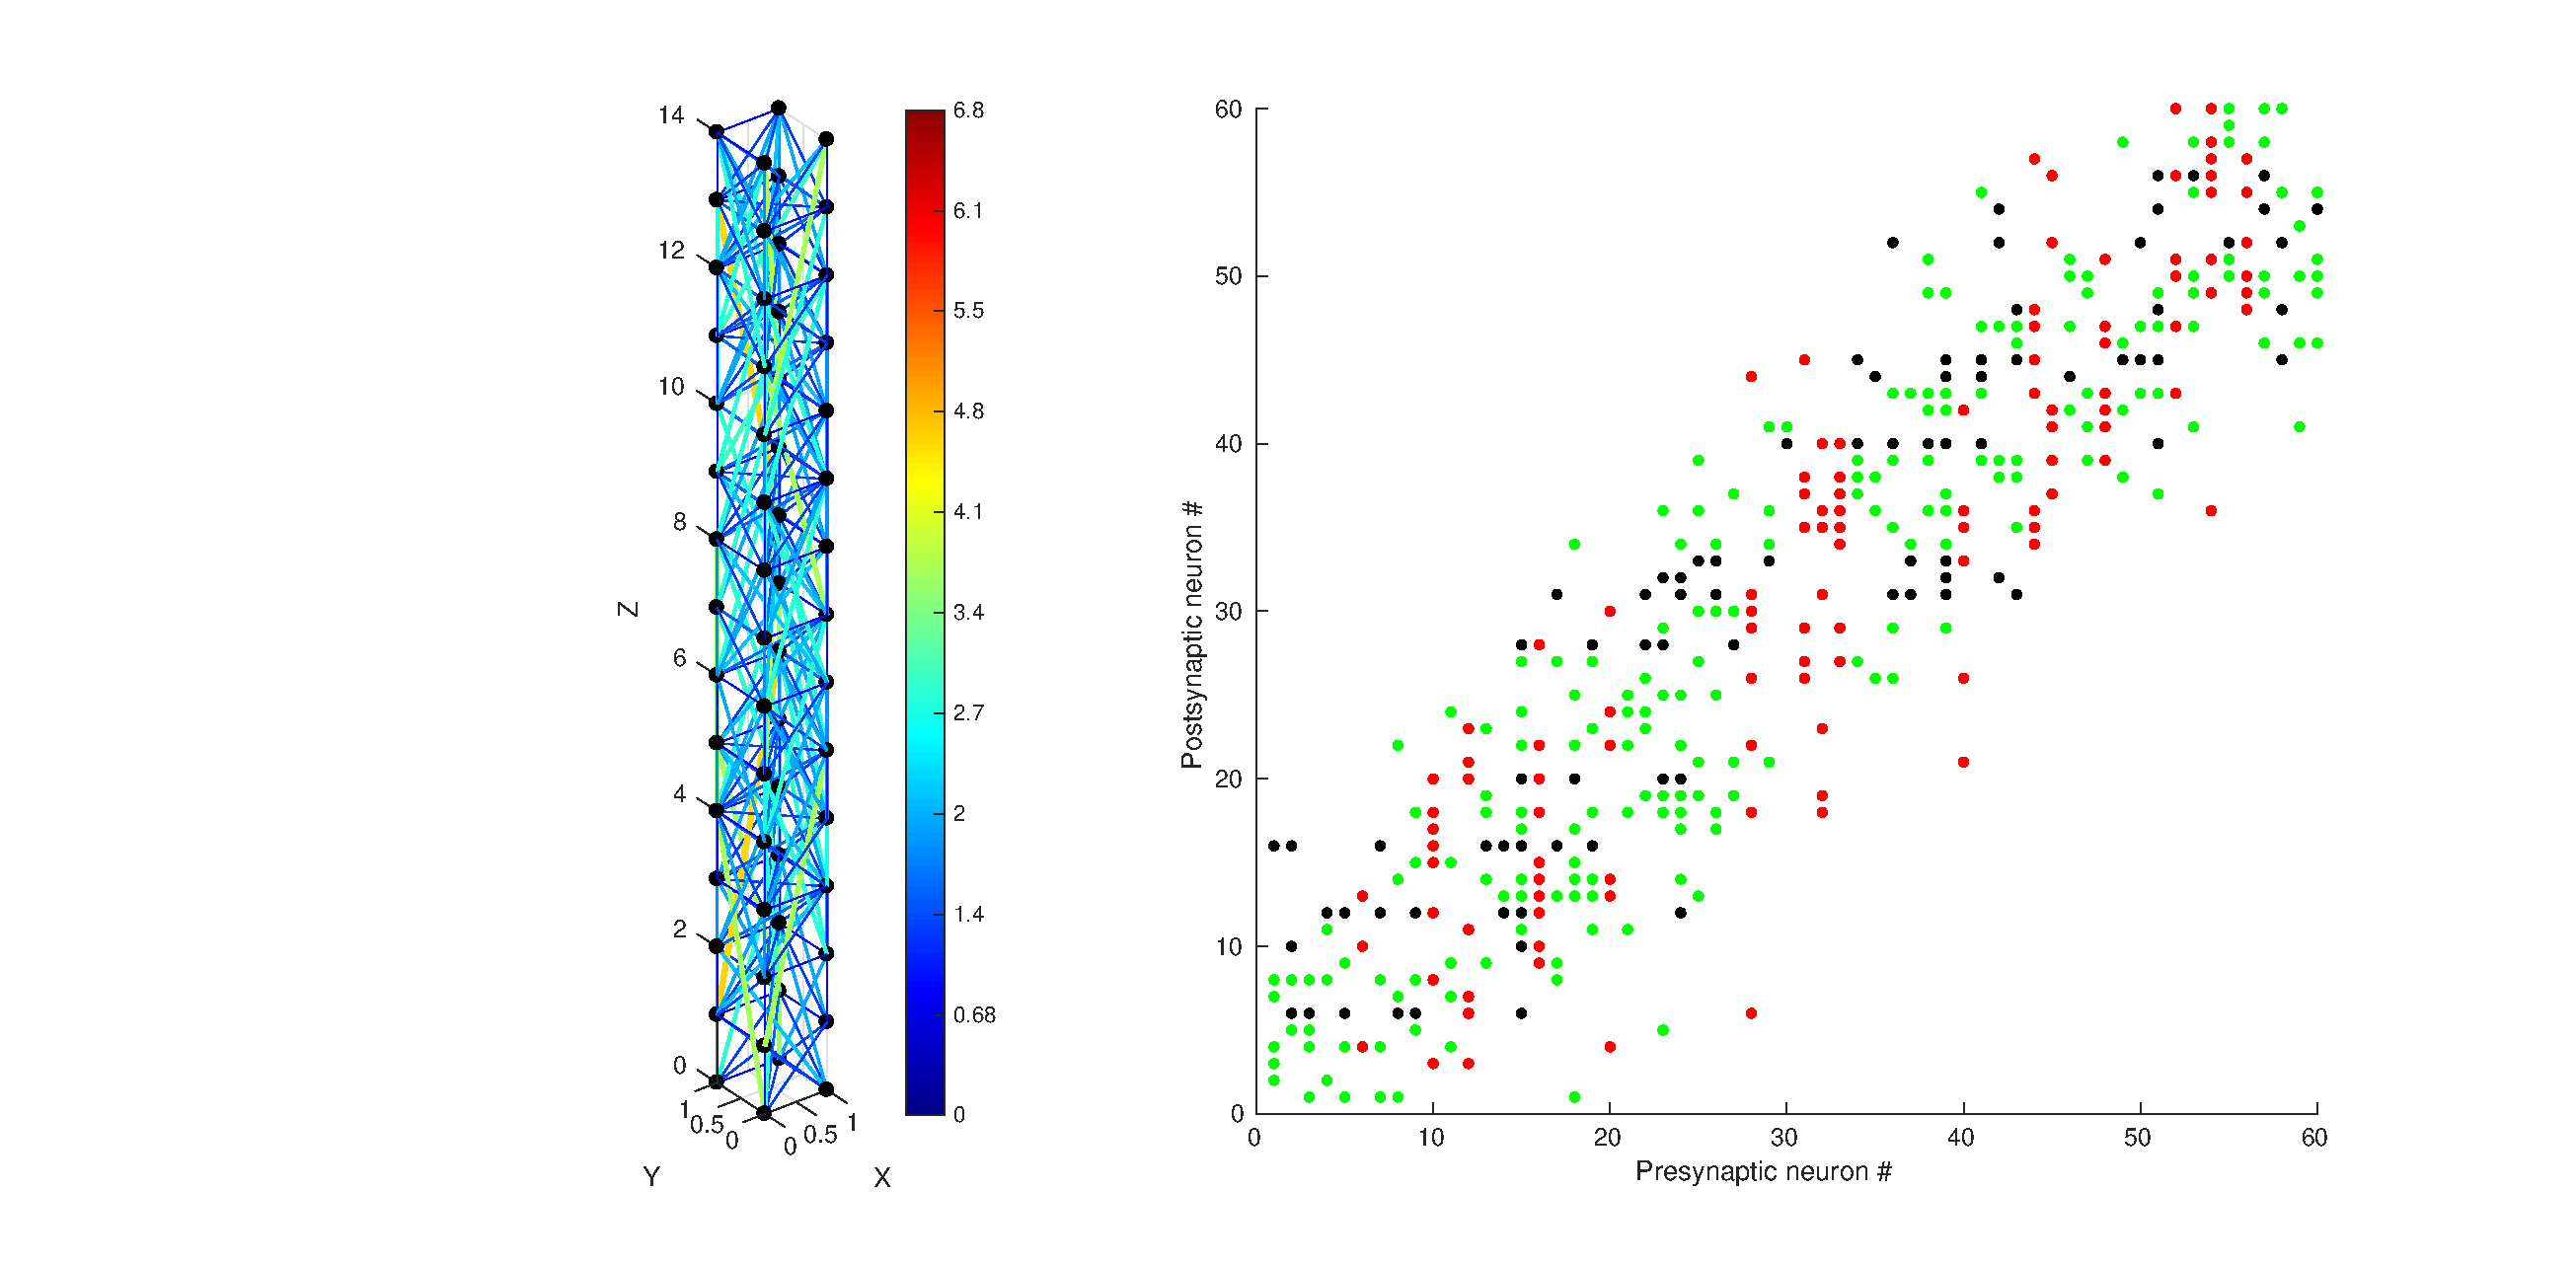
\includegraphics[width=\textwidth]{fig/column_structure}
\end{figure}

We model the firing dynamics of each neuron using the Izhikevich model \parencite{izhikevich2003} that consists of a two-dimensional model of two coupled differential equations given by:
\begin{align}
 \begin{split}
  v^\prime &= 0.04v^2+5v+140-u+I \label{eq:neuron_v} \\
  u^\prime &= a(bv-u)
 \end{split}
\end{align}
where $v$ is the membrane potential of the neuron and $u$ is a membrane recovery variable, with a spike threshold and an auxilliary after-spike resetting of parameters by:
\begin{align}
  \text{if } &v>30: v\leftarrow c, u\leftarrow u+d
\end{align}
and I is the sum of all incoming currents to the neuron, explained in detail below. 

Equation \ref{eq:neuron_v} has four parameters (a,b,c,d) that with specific values can model a wide range of neuronal spiking behavior \parencite{izhikevich2003}. 
The parameters used here (see Table \ref{tab:izzy_params}) are based on those specified in \parencite{izhikevich2003} with modification of the $c$ parameter for excitatory neurons and define a random population of neurons where $U(s,t)$ represent a number drawn from a uniform random distribution between s and t. 
\begin{table}[!htb]
 \caption{Izhikevich model parameters}
 \label{tab:izzy_params}
 \centering
 \begin{tabular}{l|c|r}
  \textbf{Parameter} & \textbf{Excitatory} & \textbf{Inhibitory} \\
  \hline
  a & 0.02 & 0.02+$\mathcal{U}$(0,0.08) \\
  b & 0.2 & 0.25-$\mathcal{U}(0,0.05)$\\
  c & -65+$\mathcal{U}(0,10)^2$ & -65 \\
  d & 8-$\mathcal{U}(0,6)$& 2 \\
 \end{tabular}
\end{table}
For solving equation (2) numerically we use the modified Euler method from \parencite{izhikevich2003} with a time step of $0.2 ms$ except were noted. 

A crucial element to evoke traveling waves in neuronal systems is the existence of time delays between the creation of a presynaptic action potential and the arrival of that spike to a target neuron. 
For this, we use distance-dependent time delays for the propagation of a spike from neuron $i$ to neuron $j$ of $\tau_{ij} = \kappa  D(i,j)$. 
The constant of porportionality $\kappa$ ranges from $0$ to $4$.
When $\kappa=0$ the action potential excites the post-synaptic neuron on the succeeding simulation time step.

The current I in equation (2) includes the sum of all incoming stimuli into neuron $i$ from other neurons $I_i$ and external stimuli $I_{i,e}$ applied to the system. 
The neuron-neuron incoming current $I_i$ into neuron $i$ is given by:
\begin{align}
 I_i(t) &= \sum_{j\ne i} \sum_{t^\prime_j} S_{ij}  \Theta(t-t^\prime_j-\tau_{ij})e^{-(\frac{t-t^\prime_j-\tau_{ij}}{\sigma_s})^2}
\end{align}

where $t'_j$ are the firing times of neuron $j$, $\Theta$ is the Heaviside step function, and the exponential factor models an exponentially decaying synapse response with a time constant of $\sigma_s = 4 ms$. 
The $S_{ij}$ represent the connection strengths between presynaptic neuron $j$ and postsynaptic neuron $i$ given by
\begin{align}
 \begin{split}
  S_{ij}^{excitatory} &= K \times \mathcal{U}\{0,0.5 \} \\
  S_{ij}^{inhibitory} &= K \times \mathcal{U}\{-1,0 \} 
 \end{split}
\end{align}

where $K$ is a parameter that modulates the strength of connections, with $K=1$ corresponding to the original model in \parencite{izhikevich2003}.

To drive the firing dynamics and create traveling waves we provide stimulation to the systems by using two different and separate external stimulus currents, $I_{i,e}$. 
One of them is a uniform background stimulus applied to each neuron $k$ that depends on whether the neuron is excitatory or inhibitory.
The stimulus values are drawn from a random distribution every $1 ms$ according to:
\begin{align}\label{eq:randomstim}
 \begin{split}
  I_k^{excitatory} &= M \times \mathcal{U}\{0,1 \} \\
  I_k^{inhibitory} &= \frac{2}{5} M \times \mathcal{U}\{0,1 \}
 \end{split}
\end{align}
where $M$ is a parameter that tunes the overall strength of the stimulus, with $M=5$ corresponding to the original model in \parencite{izhikevich2003}. 
This stimulus has the effect of creating waves that originate from any point along an SCE and one of the uses is to study interactions between multiple waves in section \ref{sub:wave_initiation}.

The other external stimulus $I_{i,e}$ is a short constant input of current applied to all of the neurons in the lowest ten layers of an SCE. 
The duration of the stimulus is $20 ms$ with a current of strength $5$ units. 
This stimulus has the effect of creating a single wave that can propagate through the total length of an SCE.
One of the uses of this stimulus is to measure the speed of the traveling wave in section \ref{sub:propagation_speed}.

For every simulation we record all of the firing events from all neurons. 
To automatically identify waves we perform a spatial clustering operation to this data to identify spatiotemporal regions identified by high firing density. 
The clustering operation produces an output cluster for any group of more than $3$ spike events that fall within a $20ms$ time window from neurons that are no more than $3$ layers apart.
Each cluster $C(t,z)$ has a time $t$ and position $z$.
This clustering removes random background firing activity. 
The waves are identified using a plane sweep algorithm that proceeds along the dimension of simulation time and applies wave labels to clusters such that all clusters with the same label are part of the same wave.
When a new cluster $C(t,z)$ is encountered, the algorithm associates $C(t,z)$ with any existing wave if the existing wave has a cluster $C(t_c,z_c)$ within $40 ms$ and $6$ units of the new cluster.
If there is no such adjacent cluster a new wave is created using $C(t,z)$ as the first cluster.
An example of the clustering and identification is shown in Figure 2.
\begin{figure}[!htb]
 \centering
 \begin{subfigure}{0.33\textwidth}
  \centering
  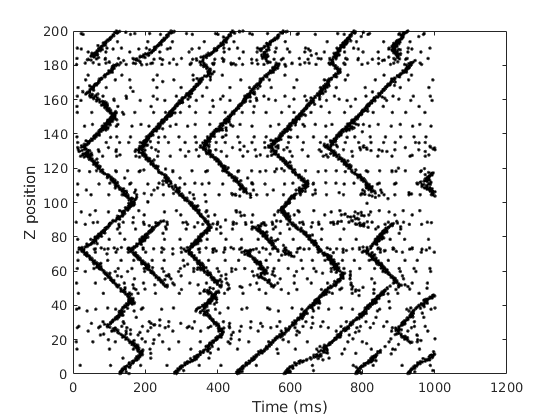
\includegraphics[width=\textwidth]{fig/2x2_firings}
 \end{subfigure}%
 \begin{subfigure}{0.33\textwidth}
  \centering
  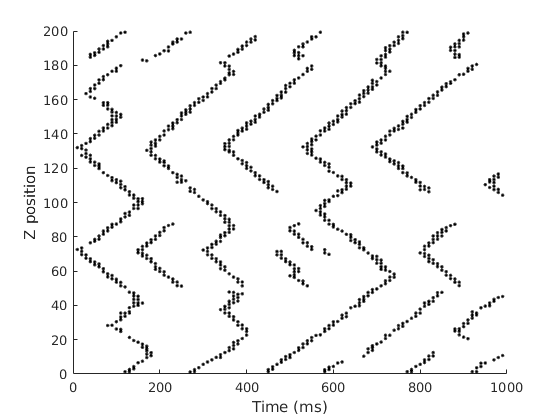
\includegraphics[width=\textwidth]{fig/2x2_density_filter}
 \end{subfigure}%
 \begin{subfigure}{0.33\textwidth}
  \centering
  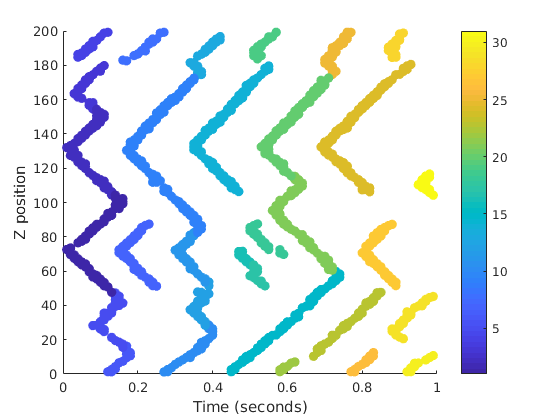
\includegraphics[width=\textwidth]{fig/2x2_wave_IDs}
 \end{subfigure}%
 \caption{Wave identification and labeling. Left: Raster plot of firing events where dots represent neuronal action potentials. 
          Traveling waves can be seen as diagonal structures of dense firing activity. 
          Center: The clustering operation removes background spikes. 
          Right: Individual waves are labeled with unique identifiers color coded in the figure.}
 \label{fig:wave_analysis}
\end{figure}

Once identified and labeled, we measure wave propagation speeds and wave initiation locations. 
We also measure the "wave firing fraction" defined as the fraction of spikes that are associated with the labeled traveling wave (total number of spikes found within the waves divided by number of spikes in the simulation). 

Our exploration of the behavior of traveling waves in an SCE involves testing properties of these waves as a function of the different parameters of our model.
We use a $2x2x50$ SCE as our ensemble.
For determining existence of traveling waves we use a background stimulation (Eq \ref{eq:randomstim}) and vary parameters around a neighborhood of the phase point $\Sigma = \{K=10,\lambda=2.5,P_{exc}=0.8,\kappa=1.0 \}$ that we have determined can sustain traveling waves.
For instances that use the step stimulus applied to the lower layers of the SCE we use $\Sigma_v = \{K=24,\lambda=2.5,P_{exc}=0.8,\kappa=1.0 \}$.
The increase in $K$ is required when using the step stimulus because the higher layers of the SCE do not receive any stimulus.
This requires stronger connections so that the traveling wave can elicit spikes from neurons resting at equilibrium.
\FloatBarrier

\section{Results}
The results are organized as a series of computational experiments on traveling waves.
We first determine which parameterizations of our model support traveling waves.
Stronger and more numerous local connections between neurons are found to facilitate the formation of traveling wave patters.
We then investigate the influence of neural dynamics and connectivity on the speed of traveling waves.
Stronger neural connections and faster action potential propagation are shown to increase traveling wave speed, but the neuron dynamics enforce an upper limit on the speed. 
Low-threshold-spiking inhibitory neurons are shown to consistently generate traveling waves through the mechanism of post-inhibitory rebound spiking.
The low-threshold-spiking inhibitory neurons also suppress traveling waves that originate from other points in the SCE.
Finally, we examine fully-connected networks and observe that traveling wave patterns can still emerge provided the action potential propagation speed is slow enough.

\subsection{Conditions for the existence of traveling waves in an SCE} \label{sub:waves}
We first explore which parameterizations of our model will support traveling waves.
We detect the waves as described in Methods, and then use the wave firing fraction metric to determine for which parameter values our model will produce traveling waves.
We fix the connection normalization constant $C$ in equation \ref{eq:connectivity} to $0.5$ and we fix the stimulus strength $M$ in equation \ref{eq:randomstim} to $5$.
The key parameters of our model that we examine are the connection strength $K$, the characteristic connection length $\lambda$, the fraction of excitatory neurons $P_{exc}$ and the delay parameter $\kappa$.

First we establish that traveling waves are observed at the fixed point $\Sigma = \{K=10,\lambda=2.5,P_{exc}=0.8,\kappa=1.0 \}$.
We then vary the individual parameters about $\Sigma$ to examine how they influence traveling wave formation.

At the fixed point $\Sigma$ the average wave firing fraction over 100 trials is found to be $88.6\%$ with a standard deviation of $4.38\%$.
A representative raster plot of the spike events (Figure \ref{fig:sigma_raster}) clearly shows the traveling waves.
\begin{figure}[!htb]
 \centering
 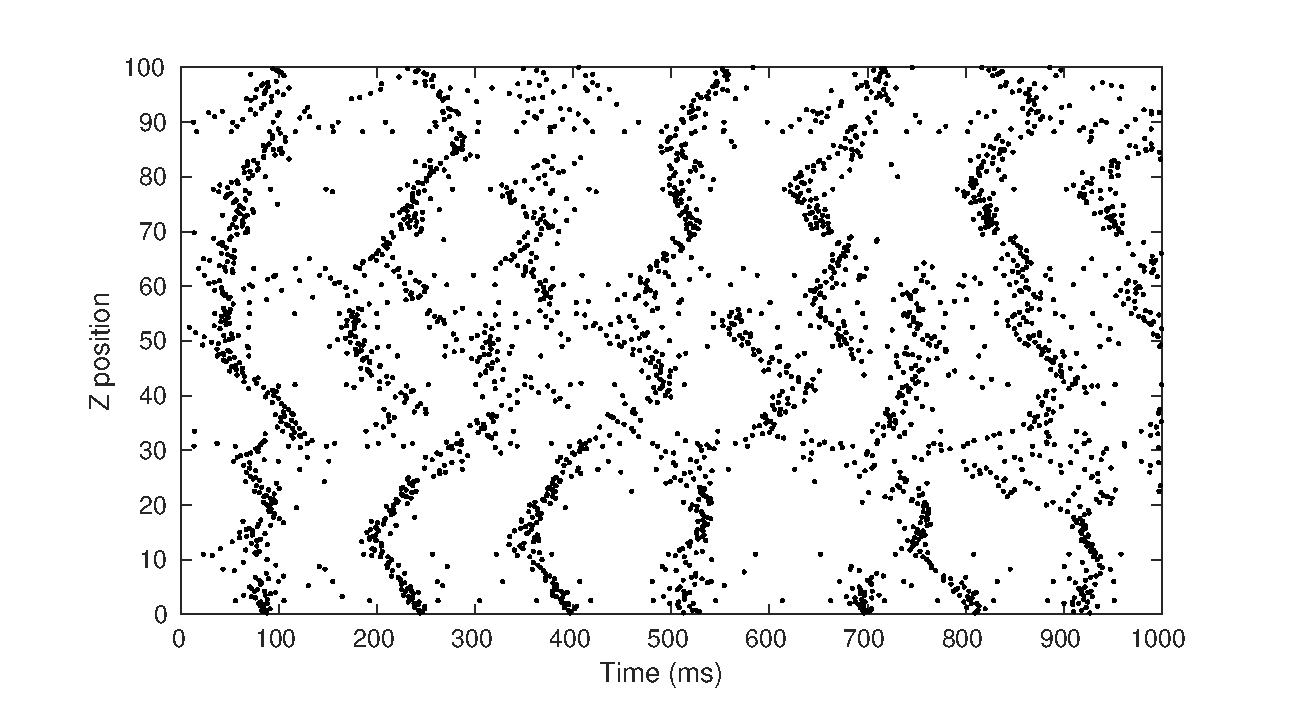
\includegraphics[width=0.75\textwidth]{fig/baseline}
 \caption{Raster plot of neuron firing events over time. The model parameters are at the fixed point $\Sigma$. Each dot represents the spike-time emission of a neuron. Traveling waves can be seen as diagonal structures of dense firing activity \parencite{Senk2018}. }
 \label{fig:sigma_raster}
\end{figure}

The effect of varying the parameters on traveling waves are shown in Figure \ref{fig:wave_parameters}.
The graphs of the wave firing fraction versus $K$, $\lambda$ and $P_{exc}$ show similar behavior.
Traveling waves are not supported for low values of these parameters.
As the parameter values increase traveling waves emerge, and as the parameters grow large the traveling waves dominate the firing activity.
Stronger connections ($K$) or more numerous connections ($\lambda$) makes it easier for firing activity to spread to adjacent neurons.
A higher excitatory fraction acts similarly to a higher connection strength. 
As the presynaptic activity to each neuron is more excitatory and less inhibitory, it is easier for the traveling wave to propagate.
These data suggest that these three parameters all work towards strengthening the local neighborhood of neurons and facilitating the propagation of coordinated spikes as traveling waves.

\begin{figure}[!htb]
 \centering
 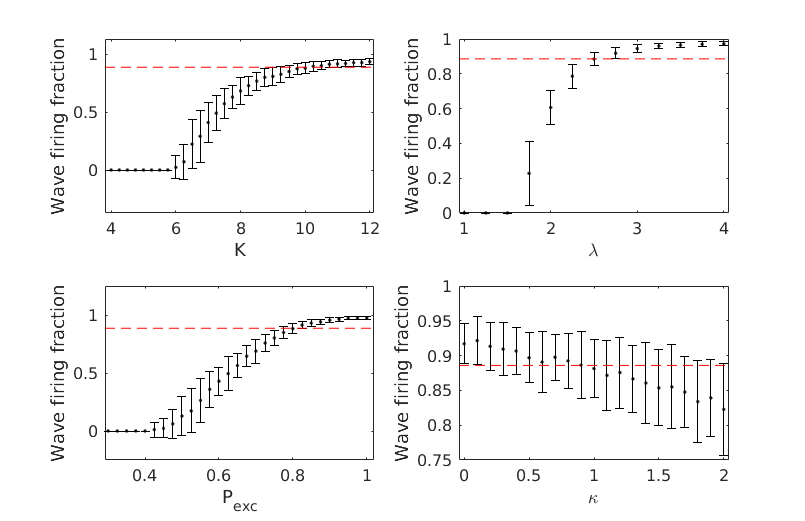
\includegraphics[width=\textwidth]{fig/ParamWaveSim}
 \caption{Onset of traveling waves as a function of model parameters in the neighborhood of $\Sigma$ (100 trials for each parameter value, error bars $1\sigma$). 
         The dashed red lines show the wave firing fraction at the fixed point $\Sigma$.  
         Varying each individual parameter while holding the other parameters at their $\Sigma$ values, we observe onset of traveling waves at $K=6$ (A), $\lambda=1.5$ (B), and $P_{exc}=0.45$ (C).  
         D) Traveling waves are present at all values of $\kappa$. }
 \label{fig:wave_parameters}
\end{figure}

\FloatBarrier

For the range of values tested, the parameter $\kappa$ does not show a strong influence on the presence of traveling waves. 
However, increasing $\kappa$ gradually reduces the fraction of neuron spikes that are associated with waves.

\subsection{Wave propagation speed} \label{sub:propagation_speed}
Cortical traveling waves have been observed with propagating speeds from $<0.1 to >0.8$ meters per second \parencite{Sato2012}\parencite{Golomb1997}\parencite{Chervin1988}.
In \parencite{Muller2018} the authors considers this consistent with the action potential propagation speeds in the gray matter of the cortex. 
We include action potential propagation in our model with a propagation time porpotional to the length of the axon.
The key elements of the dynamics include the speed at which an action potential is carried to the postsynaptic neurons, and the length of the connections.

In \parencite{Golomb1997} the authors neglected action potential propagation in their model of disinhibited cortical slices as they consider their observed wave velocity of $~0.15 m/s$ to be an order of magnitudefaster than axon potential propagation.
\parencite{Chervin1988} found even slower propagation of $0.06-0.09 m/s$ in disinhibited slices of rat cortex.
This indicates that a second key element, namely neuron amd synapse dynamics, will also influence wave propagation speed.
Biological neurons have complex internal dynamics, and will not fire instantaneously upon receiving a stimulus.
The input may push the neuron's dynamical system out of equilibrium and cause a spike, but the system dynamics take some time to evolve.
Therefore the spike will occur with some delay after the stimulus.
This is a common behavior in any multidimensional model of neuron dynamics, but it is not captured by the leaky integrate-and-fire model used in much of the previous research \parencite{keane2015}\parencite{Senk2018}.
As an example, Figure \ref{fig:delay_neuronstep} shows the delayed response of a neuron to a pulse of current using the Izhikevich model.
\begin{figure}[!htb]
 \caption{ A pulse of voltage (bottom) with magnitude $2 mV$, starting at $t=100 ms$ and lasting $2 ms$ disturbs the equilibrium membrane potential of a neuron (top), eliciting a spike at $t=112 ms$. }
 \label{fig:delay_neuronstep}
 \centering
   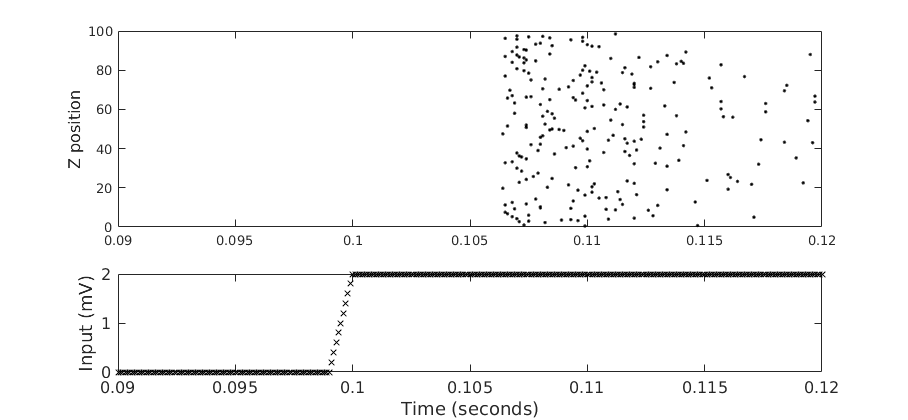
\includegraphics[width=\textwidth]{fig/WaveSpeed_NeuronStepTest}
\end{figure}

To determine this spike delay we expose populations of excitatory and inhibitory neurons to current pulses of different magnitudes.
The average firing delay of the excitatory and inhibitory neurons is shown in Figure \ref{fig:delay_neurondynamics}.
The inhibitory neurons have a lower firing threshold than the excitatory neurons \parencite{izhikevich2003} and fire with a shorter delay when given the same stimulus.
Both excitatory and inhibitory neurons exhibit a delayed response of several $ms$ or more.
\begin{figure}[!htb]
 \caption{ A stronger stimulus creates a spike with less delay. The excitatory neurons have a higher firing threshold than the inhibitory neurons and do not emit a spike for very weak stimulus.}
 \label{fig:delay_neurondynamics}
 \centering
   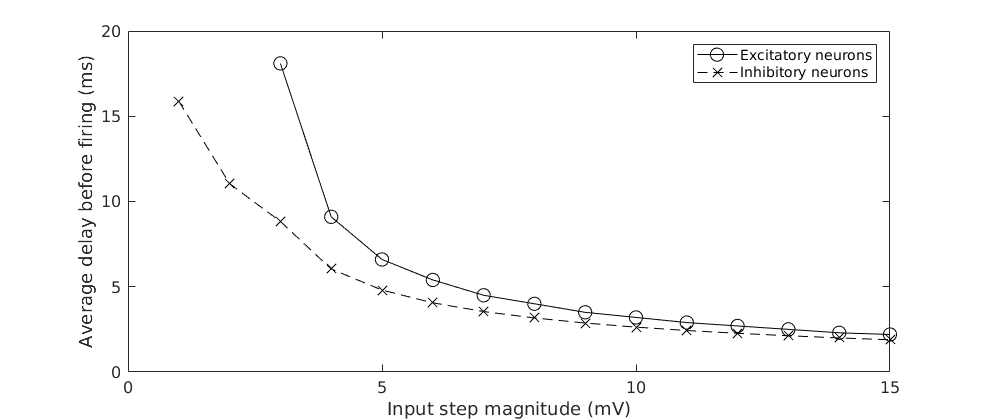
\includegraphics[width=\textwidth]{fig/WaveSpeed_NeuronDynamics}
\end{figure}

To measure wave propagation speed we use an SCE with width 2, height 2, and length 50.
Our exploration of wave speed uses a step stimulus applied to the lowest 10 layers of neurons (see Methods), while no stimulus is applied to the remaining neurons.
We then measure the time for the wave to propagate to the top layer to determine the pace in milliseconds per unit length traveled.
The speed is then calculated as the inverse of the pace in units/millisecond.

We fix the connection normalization constant $C$ in equation \ref{eq:connectivity} to $0.5$ and we fix the stimulus strength $M$ in equation \ref{eq:randomstim} to $5$ and do not vary them.
As mentioned in Methods we use $\Sigma_v$ here, with $K=24$, because the SCE cannot sustain traveling waves at $\Sigma$. 
Here, without the uniform background stimulus the neurons in the SCE are at their equilibrium point when the traveling wave arrives, and it takes a stronger stimulus from the passing wave to elicit a spike.
We increase the connection strength $K$ to provide this stronger stimulus, and find traveling waves that span the SCE starting at $K=18$. 
As $K$ increases the neurons fire with less delay, resulting in faster traveling waves (Figure \ref{fig:delay_k}).
We fix $\Sigma_v = \{K=24,\lambda=2.5,P_{exc}=0.8,\kappa=1.0 \}$ for the remainder of the wave speed computational experiments.
\begin{figure}[!htb]
 \caption{The pace (left, error bars $\pm 1 \sigma$) decreases with $K$, while the corresponding wave speed (right) increases with $K$. }
 \label{fig:delay_k}
 \centering
   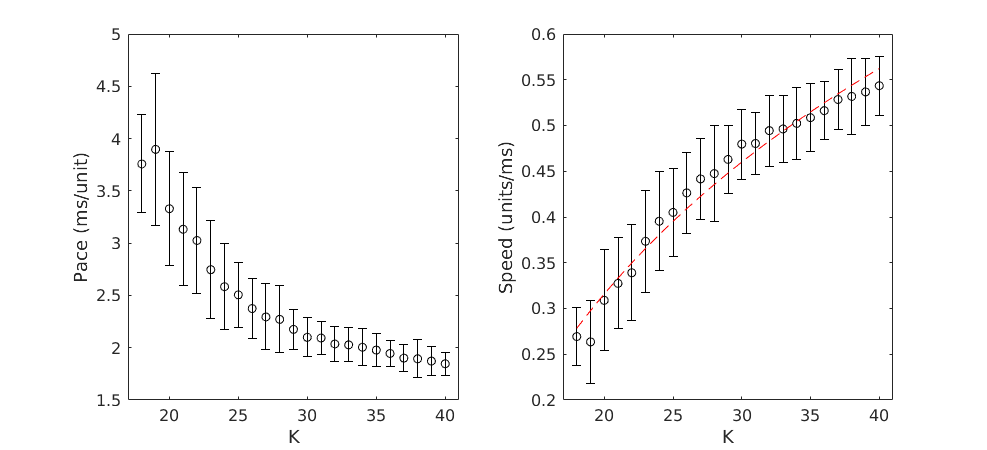
\includegraphics[width=\textwidth]{fig/WaveSpeed_K}
\end{figure}

\FloatBarrier

We next explore the influence of the action potential propagation speed, here controlled by our parameter $\kappa$, on the traveling wave propagation speed.
We vary delay parameter $\kappa$ from 0 to 5 and measure the wave pace and calculate the wave speed (Figure \ref{fig:delay_speed}).
The pace is linear in $\kappa$ as expected, but the pace does not approach $0$ as $\kappa \rightarrow 0$ due to the delayed firing inherent in the neuron dynamics.
Because each neuron does not fire instantaneously upon receiving an action potential, even instantaneous transport of action potentials does not result in a wave that can span the column instantaneously.
\begin{figure}[!htb]
 \caption{The pace (left, error bars $\pm 1 \sigma$) is linear w.r.t. $\kappa$. The intercept at $\kappa=0$ is 1.3, indicating that the neuron dynamics limit the speed of the wave. The wave speed (right) shows the expected relationship. }
 \label{fig:delay_speed}
 \centering
   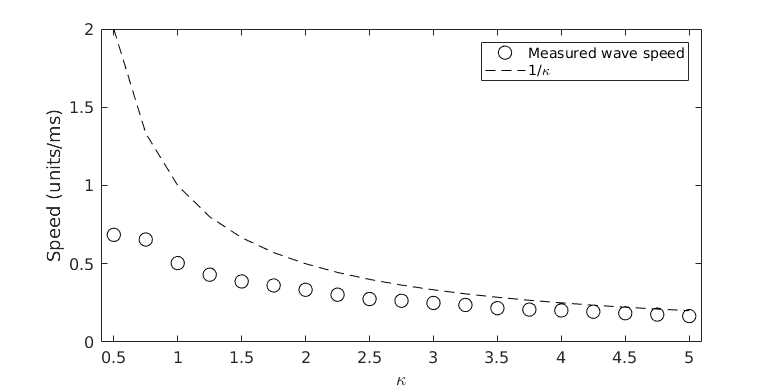
\includegraphics[width=\textwidth]{fig/WaveSpeed_Delay}
\end{figure}

\FloatBarrier

Propagation speed is also influenced by the characteristic length of the local connectivity, $\lambda$.
Since an increase in $\lambda$ results in both longer range connections, and more incoming and outgoing connections per neuron, we expect $\lambda$ to increase the wave speed through both action potential propagation and neuron dynamics.
The characteristic connection length $\lambda$ is varied from 2 to 5 and we measure the wave pace and calculate the wave speed (Figure \ref{fig:delay_lambda}).
For $\lambda<2.25$ we do not observe traveling waves.
\begin{figure}[!htb]
 \caption{ The pace (left, error bars $\pm 1 \sigma$) decreases with $\lambda$. The wave speed (right) shows that the maximum wave speed approaches $0.8$, the limit seen as $\kappa \rightarrow 0$ in Figure \ref{fig:delay_speed}. }
 \label{fig:delay_lambda}
 \centering
   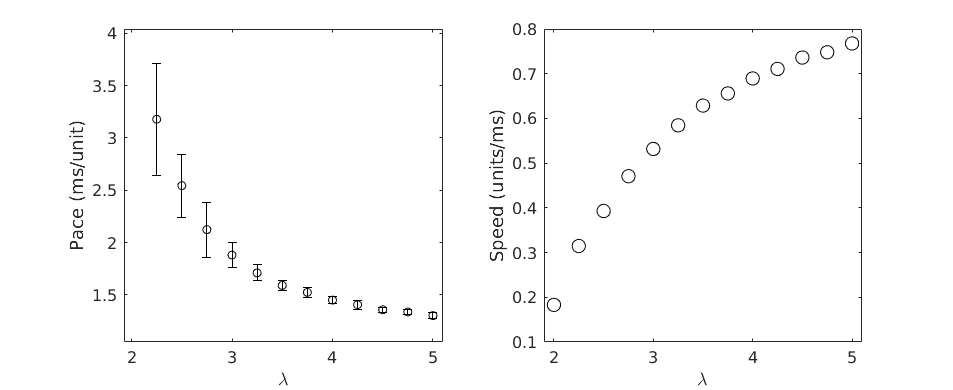
\includegraphics[width=\textwidth]{fig/WaveSpeed_Lambda}
\end{figure}

\FloatBarrier


\subsection{Wave Initiation and Density} \label{sub:wave_initiation}
Traveling waves spawned by uniform background stimulation do not appear to originate at random places in the SCE.
Instead we observe that, for a given randomly generated SCE, waves tend to spawn from certain locations within the SCE.
This is most noticeable for SCEs with very dense local connectivity with $C=1.0$ in equation \ref{eq:connectivity}.
To quantify this observation we record the initiation sites of all traveling waves that were observed in an SCE under uniform background stimulus (Figure \ref{fig:wave_initiation_sites}).
We then measure the fraction of wave initiation events (FIE) per unit length of the SCE.

\begin{figure}[!htb]
 \caption{Left: The time and place of origin of every traveling wave produced during a simulation. Right: The FIE clearly shows that traveling waves are likely to start in some regions, and unlikely to start in others.}
 \label{fig:wave_initiation_sites}
 \centering
   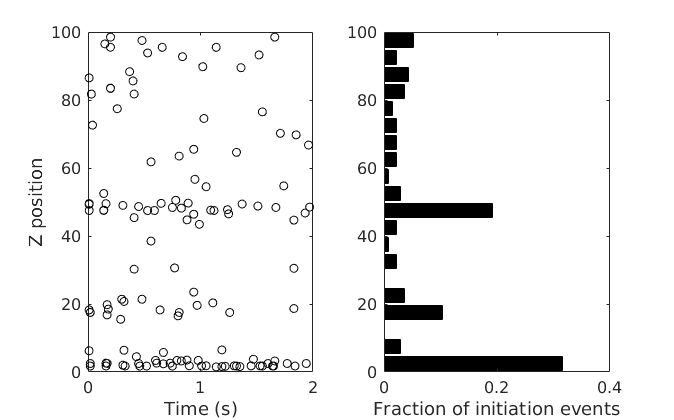
\includegraphics[width=\textwidth]{fig/InitiationSites_100sims}
\end{figure}

A separate observation is that only some of the neurons in the SCE will fire when a wave passes their location.
We observe that a single traveling wave initiated by a step stimulus can have regions of higher or lower total firing activity which we quantify by measuring the fractional number of firing events (FFE) per unit length of the SCE.
An example measurement of the firing activity in a single traveling wave is shown in Figure \ref{fig:wave_density}.
\begin{figure}[!htb]
 \caption{Density of firing events in a traveling wave initiated from a step stimulus. Left: Raster plot of the spike-emission times from a single traveling wave. Right: The FFE shows that some regions of the SCE exhibit more firing activity.}
 \label{fig:wave_density}
 \centering
   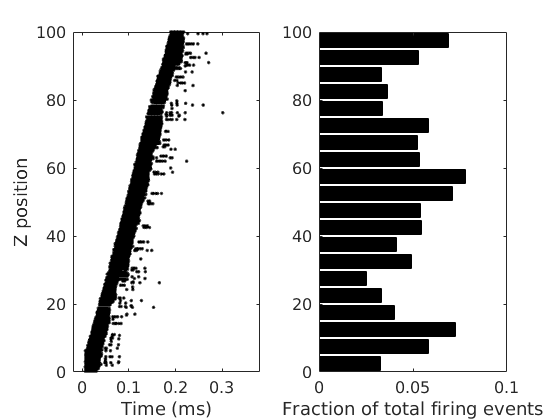
\includegraphics[width=\textwidth]{fig/ImpulseWaveDensity}
\end{figure}

By combining these two experiments we observe that the results from the FIE and the FFE appeared anti-correlated for the same SCE (see Figure S1 in Supplemental Information for examples).
To test that this observation is generally true we create 100 SCEs, apply first uniform background stimulus and then step stimulus to each SCE, and measure the correlation between the FIE and FFE (Figure \ref{fig:InitiationCorrelation}).
Although there is substantial variation between SCEs we measure a consistently negative correlation coefficient (mean $-0.26$, standard deviation $0.18$) between FIE and FFE results.
\begin{figure}[!htb]
 \centering
 \caption{Correlation between FIE and FFE for 100 different trials. }
 \label{fig:InitiationCorrelation}
 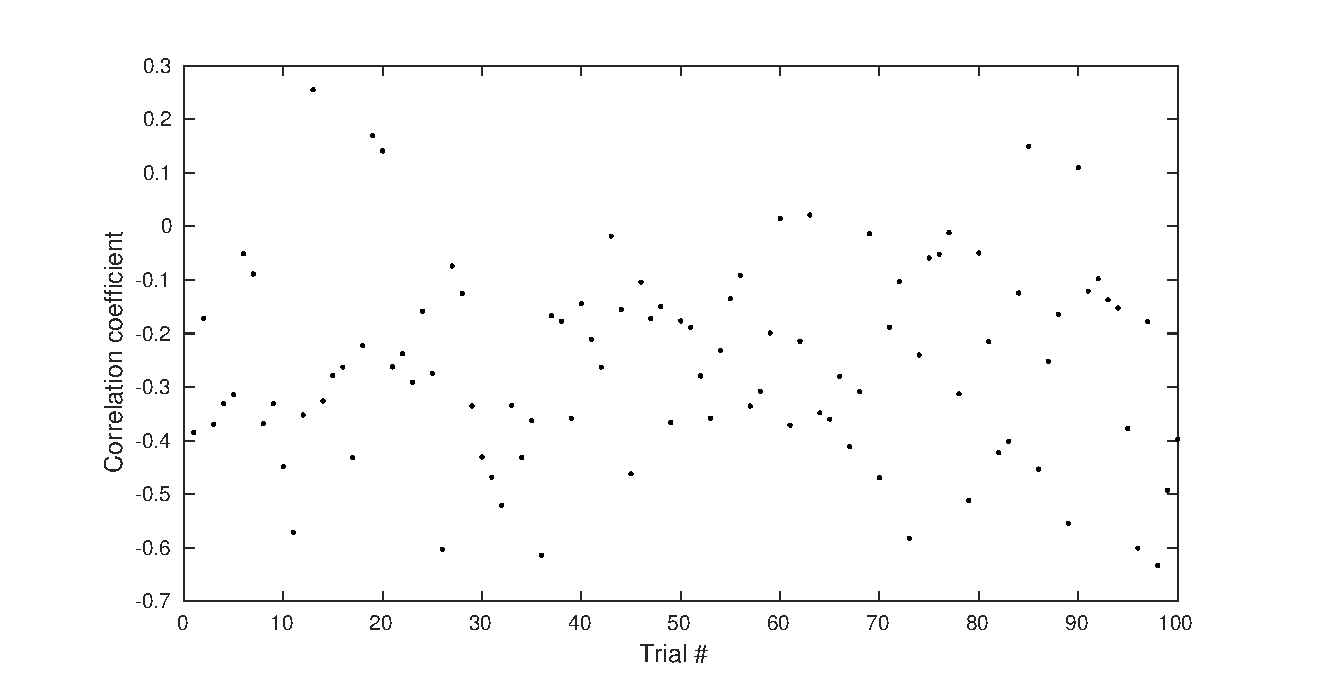
\includegraphics[width=\textwidth]{fig/InitiationCorrelation.eps}
\end{figure}

We hypothesize that these preferential wave initiation sites are created by neurons with low firing thresholds that are easy to excite.
In the Izhikevich model, inhibitory neurons can have a lower firing threshold than excitatory neurons, modeling the behavior of real inhibitory neurons in the cortex\parencite{gibson2009}\parencite{hayut2011}.
The $b$ parameter in the Izhikevich model sets the firing threshold of the individual neurons.
Neurons with higher $b$ parameter are easier to excite and therefore more likely to fire.
Per Table \ref{tab:izzy_params} excitatory neurons all have a $b$ parameter of $0.2$, while inhibitory neurons have $b$ parameters in the range $0.2-0.25$.
This indicates the preferential wave initiation sites could be due to low-threshold spiking (LTS) inhibitory neurons \parencite{izhikevich2003}.
It may seem counter-intuitive that firing activity from an \underline{inhibitory} neuron would generate traveling waves.
In fact, postinhibitory rebound spiking is observed in both cortical neurons \parencite{ascoli2010} and the Izhikevich model of neuron dynamics.
The LTS hypothesis also explains the reduced wave density at these sites.
As a traveling wave passes through the region, because of their increased activity these same inhibitory neurons suppress the surrounding neurons resulting in fewer local firing events.

A comparative computational experiment shows that low-threshold spiking inhibitory neurons can indeed generate traveling waves under background stimulus.
We first create an SCE with entirely excitatory neurons.
We then create an identical SCE except for a single LTS inhibitory neuron at $Z=50$.
The $b$ parameter of the LTS inhibitory neuron is set to $0.25$, corresponding to the lowest firing threshold used in our model.
These two SCEs are stimulated with the same uniform background stimulus. 
Figure \ref{fig:lts_inhibit} clearly shows that adding the single LTS neuron results in traveling waves emanating from $Z=50$. 
\begin{figure}[!htb]
 \caption{Simulation with a single LTS inhibitory neuron at $Z=50$. Left: an SCE with entirely excitatory neurons shows traveling waves emerging from various locations. Right: adding a single LTS neuron at $Z=50$ results in consistent wave generation from that location. }
 \label{fig:lts_inhibit}
 \centering
   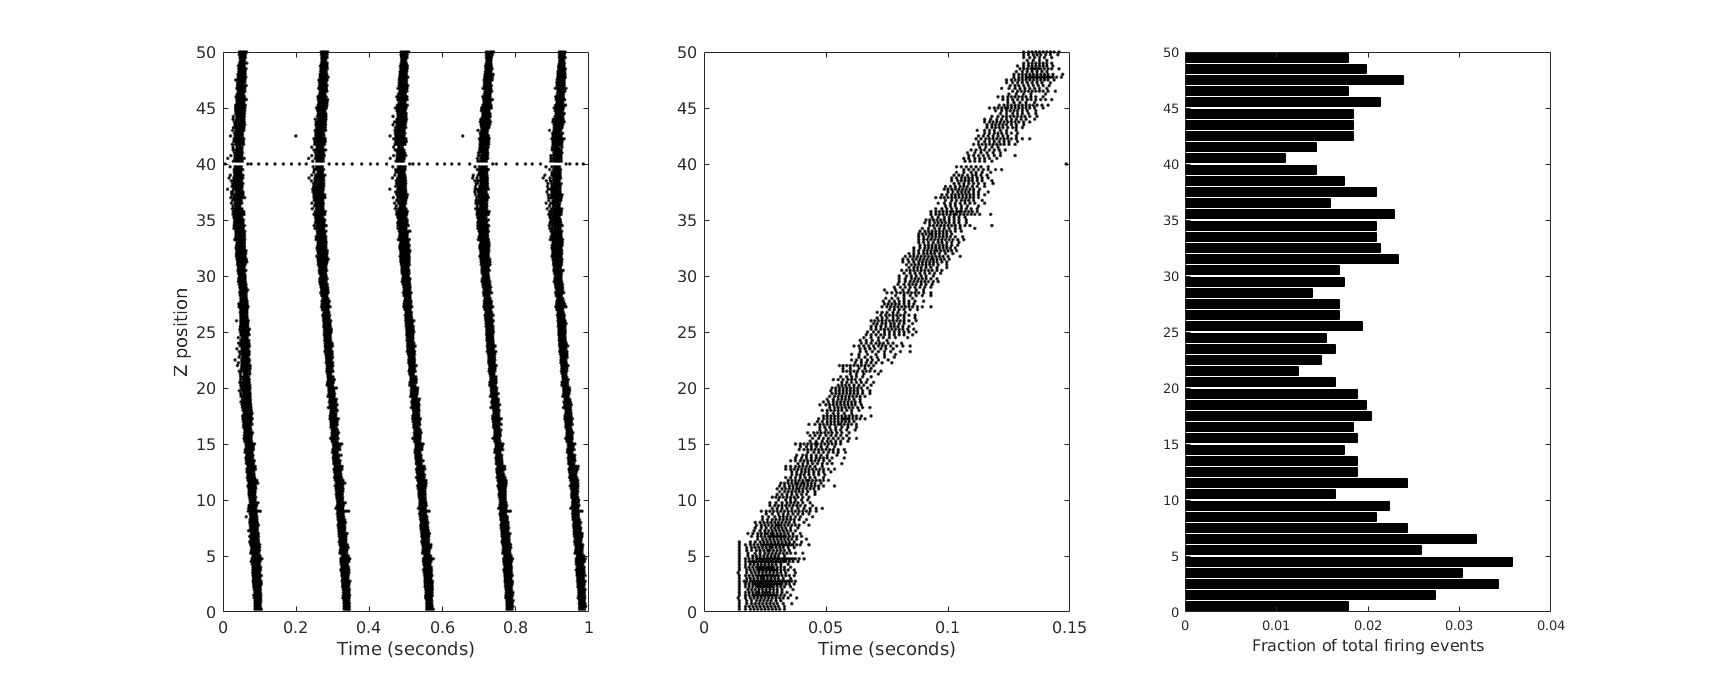
\includegraphics[width=\textwidth]{fig/SingleLTSInhibit}
\end{figure}

\FloatBarrier

\subsection{Wave patterns in fully connected networks} \label{sub:delay}
Our investigation has been concerned with traveling waves of activations that spread through locally connected networks.
We now examine whether traveling wave patterns can also be observed in fully connected networks.
We show that this is possible provided we consider the action potential propagation delay proportional to the distance between neurons, as used in all the simulations above.
We simulate an SCE with complete connectivity corresponding to $\lambda \rightarrow \infty$: all neurons are connected with probability 1 to all other neurons.
This is analogous to the original Izhikevich simulation that demonstrated synchronized firing in a completely connected neural field with random background stimulus.
We first simulate the SCE with a fixed action potential propagation delay of $1~ms$ regardless of inter-neuron distance.
The result is highly synchronized simultaneous firing among all neurons in the SCE.
We then incorporate our distance-dependent action potential propagation with the $\kappa$ parameter set to 1.
The firing is still highly synchronized, but traveling waves are now evident (Figure \ref{fig:delay_waves}).
This demonstrates that one dimensional traveling waves can emerge from fully-connected networks if the propagation delay is proportional to the inter-neuron distance.
\begin{figure}[!htb]
 \caption{Left: with global connectivity and no action potential propagation delay, the entire structure shows synchronized firing events. Right: With an action potential propagation delay, traveling waves are observed.}
 \centering
   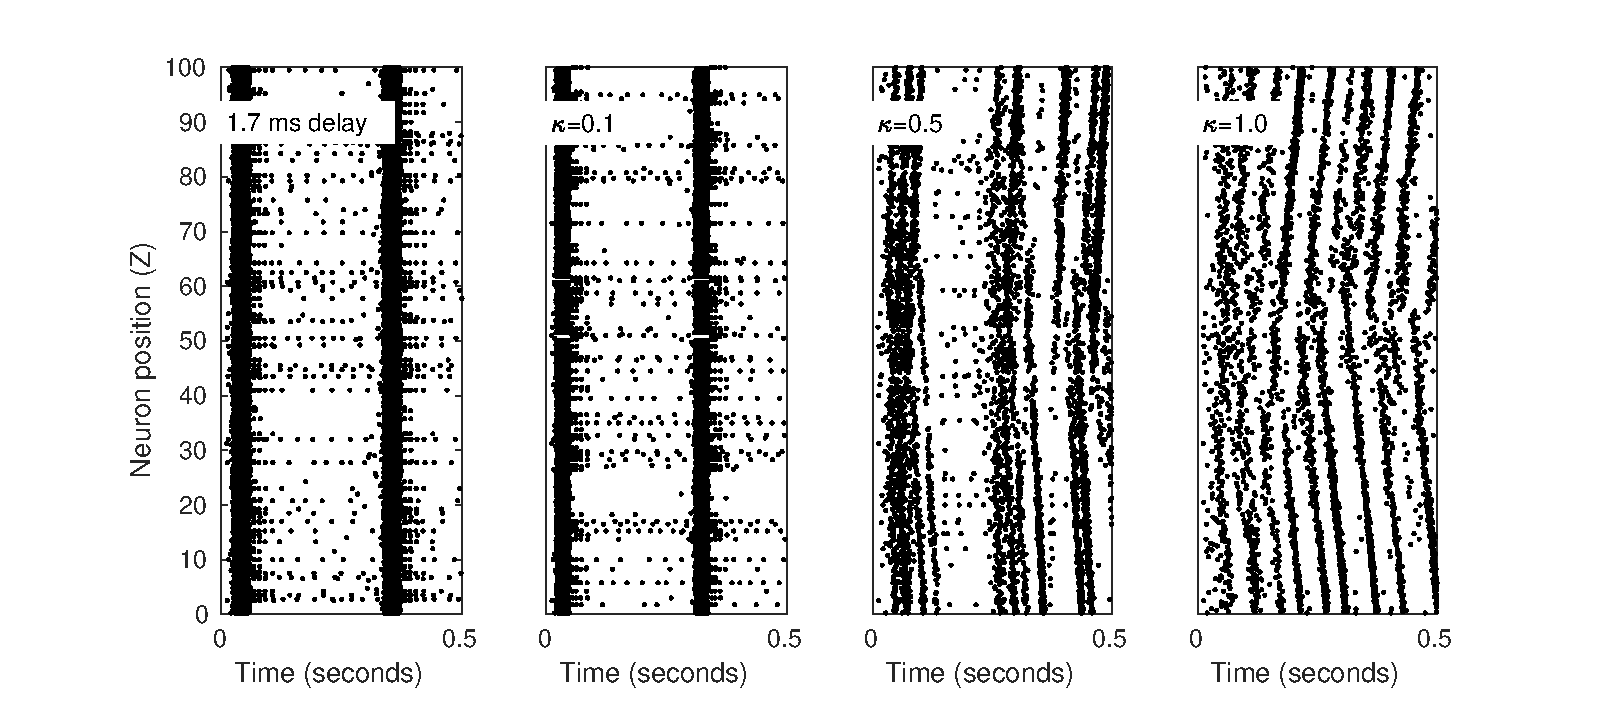
\includegraphics[width=\textwidth]{fig/DelayWaves}  
 \label{fig:delay_waves}
\end{figure}

The present case is similar to previous work (\parencite{ermentrout2001}, Figure 1) that proposed several models for traveling waves in the cortex.
The one most relevant to traveling waves in our fully-connected networks is a driving source at a spatial location that produces traveling wave patterns due to the propagation delay of action potentials.
This is a fundamentally different type of traveling wave than a chain of spike events that spreads to neighboring neurons due to local connectivity.

\section{Discussion}
We have demonstrated that representative neural structures can support traveling waves in one dimension.
Various parameters determine traveling wave formation and propagation including the connectivity, connection strength, excitatory/inhibitory balance and action potential propagation delay.
Columns with local connectivity support traveling waves, consistent with other simulations and experimental studies of cortical traveling waves.
We have also shown that  a fully-connected SCE exhibits traveling waves if the action potential propagation time depends on the inter-neuron distance. 
We have shown that the wave propagation speed depends on the action potential propagation speed.
We found that the neuron dynamics also play an important role in the wave propagation speed.
The connectivity and connection strengths influence the wave propagation speed through the neuron dynamics.
We have determined that preferential sites for wave initiation are due to the presence of inhibitory neurons with low spiking thresholds.

Previous research into traveling waves in neural networks has identified parameter regions of a neural-field model for which traveling waves exist \parencite{Senk2018}.
In this work the regions of existence were sharply defined as revealed by a linear stability analysis.
Our exploration of model parameters (Figure \ref{fig:wave_parameters}) instead shows a gradual transition region in which waves emerge and dominate the firing activity.
One possible explanation of the difference is that the previous research used highly structured spatial arrangements of excitatory and inhibitory neurons with deterministic connectivity, while our model randomly assigns neurons as excitatory or inhibitory and uses a probabilistic connection model.
Due to the stochastic nature of our model a network created with a particular set of parameters may support traveling waves in some regions while blocking traveling waves in other regions.

Other research \parencite{keane2015} has shown that complex spatial patterns emerge from two-dimensional networks of leaky-integrate-and-fire neurons when the excitation and inhibition are balanced.
In that work, when excitation dominates then only plane waves were observed instead of complex patterns.
Similarly, in one dimension we have found that traveling waves dominate the firing activity when the $P_{exc}$ grows close to $1$ (Figure \ref{fig:wave_parameters}).
Both studies show that traveling waves can become the dominant spatial pattern in excitatory networks.

We have found that low-threshold-spiking inhibitory neurons can determine the origin point of traveling waves from a uniform background stimulus.
This implies that, when no stimulus is applied, a biological neural network might have an equilibrium dynamics governed by traveling waves initiated by low-threshold-spiking inhibitory neurons.
An applied stimulus could then disturb the network from this dynamic equilibrium state.

We have found that any network with sufficiently strong connectivity and delayed action potential propagation can exhibit traveling wave structure (Figure \ref{fig:delay_waves}).
Since biological action potentials always travel with some delay, this indicates that traveling waves could be observed in the brain regardless of the inter-neuron connectivity.
The numerical results presented here could be further refined to predict biological traveling wave speed for different neuron and network parameters.
This could help distinguish between the different classes of traveling waves presented in \parencite{ermentrout2001}.

Traveling waves in one-dimensional networks have not been observed in the brain. 
Part of the reason might be that such an observation requires precise experiments that probe structures such as minicolumns in the cortex. 
These are not easy, as other properties of minicolumns are still elusive. 
However, our work shows that one-dimensional traveling waves are not only possible, but that because of the wide range of values in their allowed parameter space, their existence should be expected.


\clearpage
\printbibliography

\end{document}
